


\documentclass[letterpaper]{article}

\usepackage[utf8]{inputenc}

\usepackage{listings}
\usepackage{color}
\usepackage{graphicx}
    
%New colors defined below
\definecolor{codegreen}{rgb}{0,0.6,0}
\definecolor{codegray}{rgb}{0.5,0.5,0.5}
\definecolor{codepurple}{rgb}{0.58,0,0.82}
\definecolor{backcolour}{rgb}{0.95,0.95,0.92}

%Code listing style named "mystyle"
\lstdefinestyle{mystyle}{
  backgroundcolor=\color{backcolour},   commentstyle=\color{codegreen},
  keywordstyle=\color{magenta},
  numberstyle=\tiny\color{codegray},
  stringstyle=\color{codepurple},
  basicstyle=\footnotesize,
  breakatwhitespace=false,         
  breaklines=true,                 
  captionpos=b,                    
  keepspaces=true,                 
  %numbers=false,                    
  numbersep=5pt,                  
  showspaces=false,                
  showstringspaces=false,
  showtabs=false,                  
  tabsize=2
}

%"mystyle" code listing set
\lstset{style=mystyle}

\usepackage[letterpaper,margin=1.75in,noheadfoot]{geometry}
\usepackage{fontspec, color, enumerate, sectsty}
\usepackage[normalem]{ulem}
\usepackage{amsmath}
\usepackage{listings}

\newcommand{\reporttitle}{An Introduction to Git}
\newcommand{\name}{By Shiva Bhusal}
\newcommand{\course}{}

\usepackage[bookmarks, colorlinks, breaklinks,
pdftitle={\name - \reporttitle},pdfauthor={\name}, unicode]{hyperref}

\hypersetup{
    colorlinks=true,
    linkcolor=blue,
    filecolor=magenta,      
    urlcolor=cyan,
    pdftitle={Sharelatex Example},
    bookmarks=true,
    pdfpagemode=FullScreen,
    }

\usepackage{hyperref}


%%% Start of our document 

\begin{document}
\begin{center}{\huge \scshape \reporttitle}\end{center}
\begin{center}\vspace{0.2em} {\Large \name\\}
  {\course}\end{center} 
  
\tableofcontents
  
\section{Introduction}
\textit{Git} is a distributed version control system which can serve as a better alternative to centralized version control systems like \textit{TFS} and \textit{SVN}. There are many advantages of Git over the centralized version control systems which can be summarized in the following points:
\begin{itemize}
    \item It is distributed.So,each developer has a full copy of the repository.
    \item It handles complex merges faster.
    \item \textit{Git} is comparatively easier and less complicated for collaborative development, especially involving thousands of developers.
    \item Branching is cheap and switching between branches is easy.
    \item In general, it provides more functionality and control than the centralized version control systems.
\end{itemize}

Besides, most of the open source projects use \textit{Git} as the version control system. So, if you are interested in open source projects, you are expected to know the basics of \textit{Git}.In this tutorial, you will learn how to install and setup \textit{Git} and use it as a version control system for your projects. 

\section{Installation and setup}
Git can be downloaded and installed by following the instructions in the link below.\\

%\begin{lstlisting}[language=Bash]
\url{https://git-scm.com/downloads}
%\end{lstlisting}
\\

After you install \textit{Git}, create an account on \href{https://github.com/}{Github} or \href{https://about.gitlab.com/}{Gitlab}.

If you are using a Unix system, please use the bash terminal to run the git commands. If you are using Windows, you can use Git Bash.

Then, set up your identity in the computer you have installed \textit{Git}. This will make sure that every time you make the changes and push your changes, the change is associated with you as an author. \\

\begin{lstlisting}[language=Bash]
git config --global user.name "Jane Doe"
\end{lstlisting}

\begin{lstlisting}[language=Bash]
$ git config --global user.email "jane.doe@gmail.com"
\end{lstlisting}

After you have setup everything mentioned above, create a repository and refer to the basic Git commands in section 3 to get started. 

\section{Basic Git Commands}
Below are some of the useful Git commands, with corresponding examples:

\subsection{git clone}
\begin{lstlisting}[language=Bash]
git clone https://github.com/shivapbhusal/git-demo.git
\end{lstlisting}
It creates the local copy of the repository. In the example below, we are creating a local copy of the repository \textit{git-demo}.

 \begin{figure}[h]
    \centering
    \frame{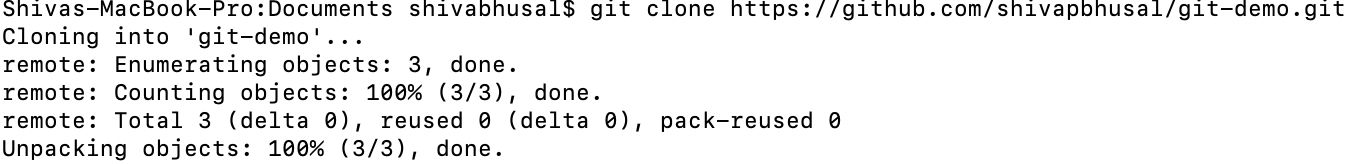
\includegraphics[scale=0.56]{figure/clone.png}}
    \caption{Cloning the demo repository}
  \end{figure}

\subsection{status}
Gives the current status of the files in the local repository. The command below shows that there is an un-tracked file called \textit{foo.py} which has been created recently.

\begin{lstlisting}[language=Bash]
git status
\end{lstlisting}

\begin{figure}[h]
    \centering
    \frame{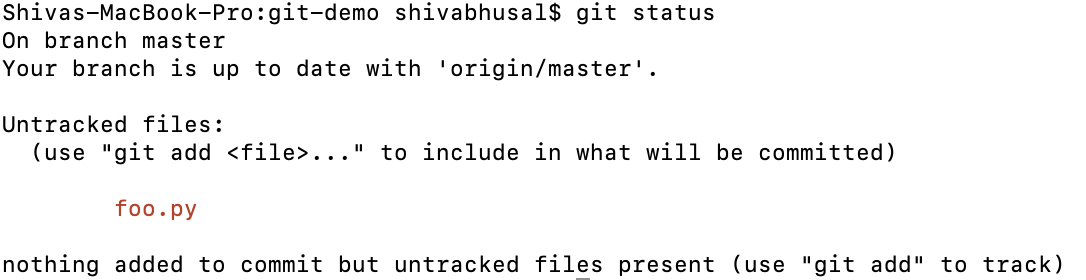
\includegraphics[scale=0.7]{figure/status.png}}
    \caption{Git status after creating one file called foo.py}
  \end{figure}


\subsection{add}
Adds the changes for staging. In other words, this command decides which changes in the current version of the repository will go into the next version.
\begin{lstlisting}[language=Bash]
git add foo.py
\end{lstlisting}

\subsection{commit}
Confirms the changes in the local repository. Creates a new version of the repository incorporating the local changes.

\begin{lstlisting}[language=Bash]
git commit -m "add foo.py"
\end{lstlisting}

\begin{figure}[h]
    \centering
    \frame{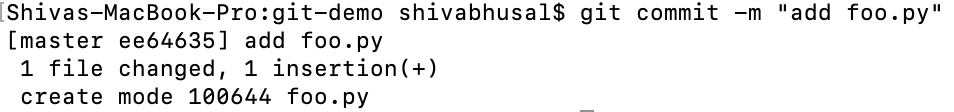
\includegraphics[scale=0.8]{figure/commit.png}}
    \caption{Git commit operation}
  \end{figure}


\subsection{push}
Merges the locally committed changes with the repository in the remote server.

\begin{lstlisting}[language=Bash]
git push
\end{lstlisting}

\begin{figure}[h]
    \centering
    \frame{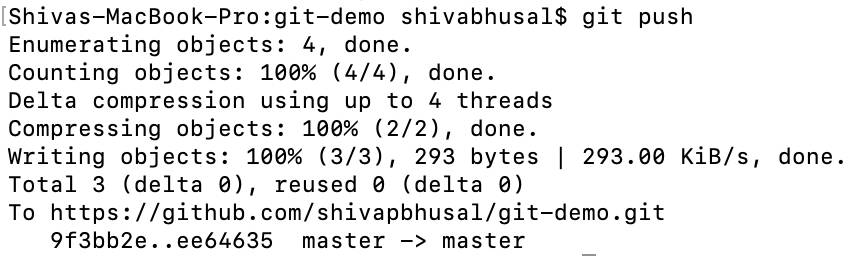
\includegraphics[scale=0.7]{figure/push.png}}
    \caption{Git commit operation}
  \end{figure}

\subsection{pull}
Let's assume, another member of the team has already pushed the changes. In such a case, we do git pull to get the latest changes in the repository. 

\begin{lstlisting}[language=Bash]
git pull
\end{lstlisting}

\begin{figure}[h]
    \centering
    \frame{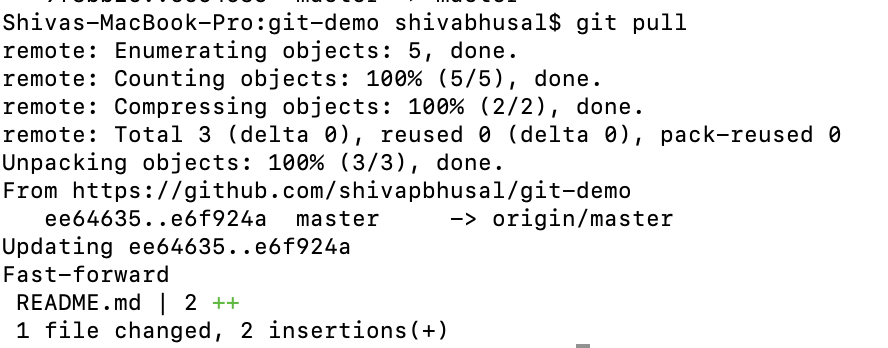
\includegraphics[scale=0.7]{figure/pull.png}}
    \caption{Git pull operation}
  \end{figure}


\subsection{branch}
Creates a new branch. In this example, a new branch of test\_branch is created. 

\begin{lstlisting}[language=Bash]
git branch dev
\end{lstlisting}

\subsection{checkout}
Switches from the current branch to the specified branch.

\begin{lstlisting}[language=Bash]
git checkout dev
\end{lstlisting}

Now, we are switched from the master branch to the dev branch.


\subsection{stash}
Ignores ( undoes) the uncommitted changes made in the local.
\begin{lstlisting}[language=Bash]
git stash
\end{lstlisting}

\begin{figure}[h]
    \centering
    \frame{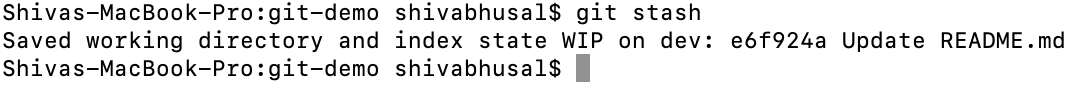
\includegraphics[scale=0.7]{figure/stash.png}}
    \caption{Git stash operation}
  \end{figure}





\subsection{merge}
\begin{lstlisting}[language=Bash]
git merge origin/dev
\end{lstlisting}
Merges the changes of the specified branch with the current branch. In this example, the changes committed in the test\_branch are merged with the master branch. 

\begin{figure}[h]
    \centering
    \frame{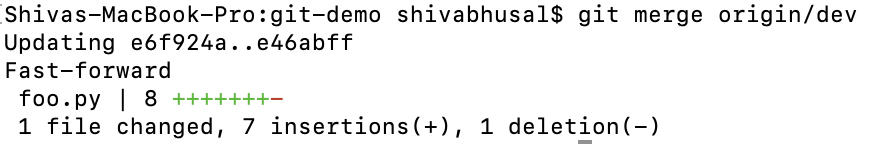
\includegraphics[scale=0.7]{figure/merge.png}}
    \caption{Git merge operation}
  \end{figure}

\subsection{log}
Displays the version history of the repository or the list of the historical commits. 
\begin{lstlisting}[language=Bash]
git log
\end{lstlisting}

\section{Using .gitignore}
It is not a good practice binary files and executable. You may also want to exclude some directories of your project from the staging. In order to exclude the selective files, a \textit{.gitignore} file can be used.

This will make sure that any file with extension \textit{.log} is ignored while performing the \textit{Git} operations. 

\end{document}

%%% End of our document 